\documentclass{beamer}
\usepackage{listings}
\lstset{
%language=C,
frame=single, 
breaklines=true,
columns=fullflexible
}
\usepackage{subcaption}
\usepackage{url}
\usepackage{amsmath}

\usepackage{amsthm}

\usepackage{tikz}
\usepackage{graphicx}
\usepackage{tkz-euclide} % loads  TikZ and tkz-base
%\usetkzobj{all}
\usetikzlibrary{calc,math}
\usepackage{float}

\newcommand\norm[1]{\left\lVert#1\right\rVert}
\renewcommand{\vec}[1]{\mathbf{#1}}
\newcommand{\R}{\mathbb{R}}
\newcommand{\C}{\mathbb{C}}
\providecommand{\brak}[1]{\ensuremath{\left(#1\right)}}
\providecommand{\abs}[1]{\vert#1\vert}
\providecommand{\fourier}{\overset{\mathcal{F}}{ \rightleftharpoons}}
\newcommand{\myvec}[1]{\ensuremath{\begin{pmatrix}#1\end{pmatrix}}}
\providecommand{\mean}[1]{E[ #1 ]}
\providecommand{\sbrak}[1]{\ensuremath{{}\left[#1\right]}}
\providecommand{\cbrak}[1]{\ensuremath{\left\{#1\right\}}}
\usepackage[export]{adjustbox}
\usepackage[utf8]{inputenc}
\usepackage{amsmath}
\usetheme{Boadilla}
\title{Probability Analysis of Age of Information in Multi-hop Networks}
\author{Rachapalle Shashank Anirudh}
\institute{CS20BTECH11040}
\date{\today}

\begin{document}
\begin{frame}{}
 \titlepage 
\end{frame}
\begin{frame}{Introduction}
$\bullet$AGE OF information (AoI) is a metric that measures the
information freshness from the perspective of the receiver
monitoring a remote process. It is defined as the elapsed time
since the generation of the freshest packet at the receiver.\\
$\bullet$AoI increases until the arrival of a fresher status update at the
receiver and drops upon its successful reception. Therefore,
receiving status updates regularly plays a key role in sustaining
information freshness.\\
$\bullet$In addition, the staleness of a newly
received update is characterized by the time it has spent in
the network to reach the destination. As a result, a good AoI
performance is achieved when status updates are delivered not
only regularly but also timely.
\end{frame}

\begin{frame}{Key words}
$\bullet$Peak AoI\\
$\bullet$preemptive Last Generated First Served (PLGFS)\\
$\bullet$Sampling Event\\
$\bullet$Sampling Period\\
\end{frame}

\begin{frame}{}
Our main motive for this work is:\\
$\bullet$we consider a N-hop network with time-invariant packet loss probabilities on each
link.\\
$\bullet$We derive closed form equations for the probability mass
function of AoI.\\
\end{frame}
\begin{frame}{system model}
$\bullet$We consider a physical process located at the source node generating status updates periodically and a monitor located at the receiver node. The source and receiver nodes are N-hops
away from each other.\\
$\bullet$Each transmitter over the path, i.e., the source and the
intermediate relay nodes, discards any older packet in the
transmission queue upon the arrival of a new update. \\
$\bullet$Each link n is prone to packet loss with time-invariant failure probability, i.e.,$p_{n}(t)=p_{n}, \forall t$ . \\
$\bullet$Time is divided into slots of length $t_{s}$ which is also the smallest time unit in our model. Each packet transmission starts at the beginning of a slot and completes within the same slot.\\
\end{frame}


\begin{frame}{}
    \begin{figure}[h]
    \centering
    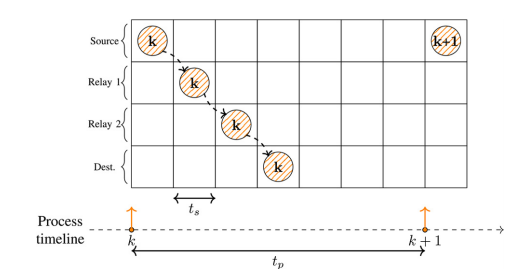
\includegraphics[width=1\textwidth]{pic1.PNG}
\end{figure} 
\end{frame}


 \begin{frame}
   \begin{figure}[h]
    \centering
    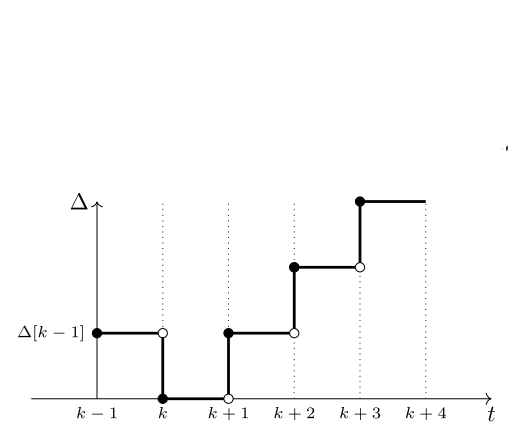
\includegraphics[width=0.8\textwidth]{pic 2.PNG}
\end{figure}   
 \end{frame}


\begin{frame}{Analysis}
Let $\gamma_{n}[k] \in \{0, 1\}, n \in \{1, 2,..., N \}$, indicate the outcome
of the transmission on the n-th link in sampling period k with
$Pr[\gamma_{n}[k] = 1] = 1-p_n, \forall k$. Furthermore, let $ \Delta_n[k], n \in
\{0, 1, 2,..., N \}$, be the AoI at hop n after the transmission
slot that is allocated to the previous link.\\
\begin{align}
\Delta_n[k]=
\begin{cases}
 \Delta_{n-1}[k]&\gamma_n[k]=1\\
 \Delta_{n}[k-1]+1 &\gamma_n[k]=0
\end{cases}
\end{align}
\end{frame}

\begin{frame}{}
   $\bullet$ we begin with a simple single hop network.\\
   The failure probability on the first link is denoted with
$p_1 \in [0, 1]$. Thus, the probability of the AoI at the relay being
$\delta_1 \in Z\geq 0$ can be written as:\\
\begin{align}
    Pr[\Delta_1[k] = \delta_1] &= (1-p_1) · p_1^{\delta_1} \forall k\\
    E[\Delta_1]&=\sum_{\delta_1=0}^\infty Pr[\Delta_1[k]=\delta_1].\delta_1\\
    &=\frac{p_1}{1-p_1}
    \end{align}
    $\bullet$ Now we consider a 2 hop network\\
    $\bullet$The loss probabilities on two links are independent, we can treat each link independently.\\
    $\bullet$The contribution of the source-to-relay link to $\Delta_1$, is analogous to the single-hop case. However, in contrast to the source
node, the information at the relay is now $\delta_1$ periods old.\\
\end{frame}

\begin{frame}{}
 \begin{align}
\Delta_{n-1}[k_n] &= \delta_{n-1}\\
 Pr[\Delta_2[k] &= \delta_2 | \Delta_1[k_2] = \delta_1]=
 \begin{cases}
  0&\delta_2 < \delta_1\\
  (1-p_2)p_2^{\delta_2-\delta_1} &\delta_2 \geq\delta_1
 \end{cases}
 \end{align}
\begin{align}
Pr[\Delta_2[k] &= \delta_2] =\sum_{\delta_1=0}^{\delta_2}
Pr[\Delta_2[k] = \delta_2 | \Delta_1[k_2] = \delta_1]
\times Pr[\Delta_1[k_2] = \delta_1]\\
Pr[\Delta_2[k] = \delta_2] &=(1-p_1)(1-p_2).\frac{p_2^{\delta_2+1}-p_1^{\delta_2+1}}{p_2-p_1}\\
E[\Delta_2]&=\frac{p_1}{1-p_1}+\frac{p_2}{1-p_2}
\end{align}
\end{frame}

\begin{frame}{Age at nth link}
$\bullet$ we extend our results to n-hop\\
\begin{multline}
    Pr[\Delta_n[k] = \delta_n]& =\sum_{\delta_{n-1}=0}^{\delta_n}
Pr[\Delta_n[k] = \delta_n | \Delta_{n-1}[k_n] = \delta_{n-1}]
\times Pr[\Delta_{n-1}[k_n] = \delta_{n-1}], \forall k\\
\end{multline}
$\bullet$Closed form for higher number of hops can also be obtained
using a similar analysis. For instance for 3-hops we obtain:\\
\begin{align}
    Pr[\Delta_3[k]=\delta_3]=\frac{\prod_{i=1}^3(1-p_i)}{p_2-p_1}\sum_{j=1}^2(-1)^j.p_j.\frac{p_3^{\delta_3+1}-p_j^{\delta_3+1}}{p_3-p_j}
\end{align}
\end{frame}

\begin{frame}{Simulation}
   $\bullet$. Each scenario is simulated for $T_{sim} = 100 000$ sampling periods and
repeated 100 times\\
$\bullet$We measure the expected AoI as:\\
\begin{align}
    E[\Delta_3]&=\frac{1}{T_{sim}}\sum_{k=1}^{T_{sim}}\Delta_3[k]
\end{align}
   $\bullet$ we can also use\\
\begin{align}
    E[\Delta_3]&=\sum_{i=1}^3\frac{p_i}{1-p_i}
\end{align}
\end{frame}

\begin{frame}{}
  \begin{figure}[h]
    \centering
    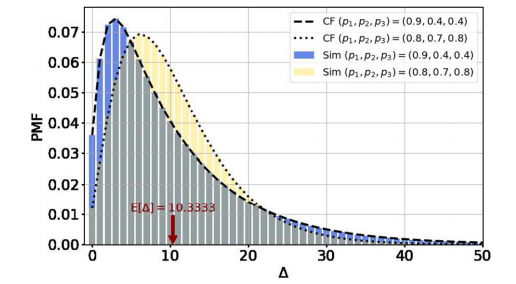
\includegraphics[width=0.8\textwidth]{pic 4.PNG}
\end{figure}
\end{frame}
\end{document}